\documentclass{standalone}
\usepackage{tikz}
\usetikzlibrary{arrows.meta, positioning, shapes}

\begin{document}

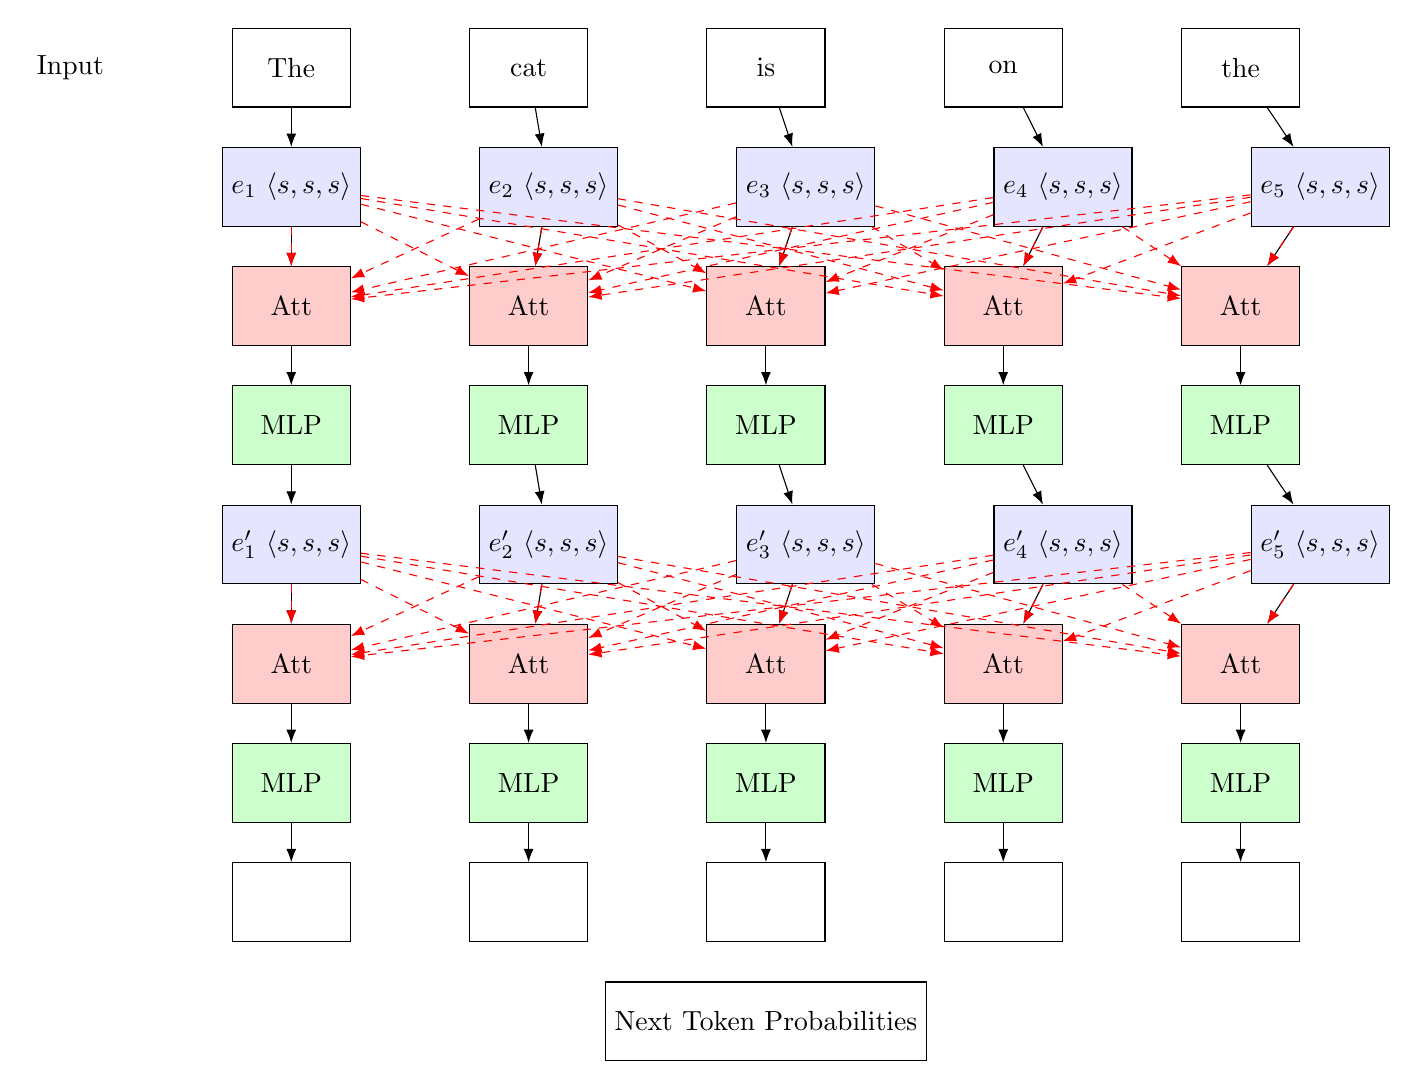
\begin{tikzpicture}[
    node distance=0.5cm and 1.5cm,
    box/.style={draw, rectangle, minimum height=1cm, minimum width=1.5cm},
    att/.style={box, fill=red!20},
    mlp/.style={box, fill=green!20},
    emb/.style={box, fill=blue!10},
    arr/.style={-Latex, red, dashed}
]

% Input
\node (input) {Input};
\node[right=of input, box] (w1) {The};
\node[right=of w1, box] (w2) {cat};
\node[right=of w2, box] (w3) {is};
\node[right=of w3, box] (w4) {on};
\node[right=of w4, box] (w5) {the};

% Initial Embeddings
\node[below=of w1, emb] (e1) {$\boldsymbol{e}_1$ $\langle s, s, s \rangle$};
\node[emb, right=of e1] (e2) {$\boldsymbol{e}_2$ $\langle s, s, s \rangle$};
\node[emb, right=of e2] (e3) {$\boldsymbol{e}_3$ $\langle s, s, s \rangle$};
\node[emb, right=of e3] (e4) {$\boldsymbol{e}_4$ $\langle s, s, s \rangle$};
\node[emb, right=of e4] (e5) {$\boldsymbol{e}_5$ $\langle s, s, s \rangle$};

% Layer 1
\node[att, below=of e1] (a11) {Att};
\node[att, right=of a11] (a12) {Att};
\node[att, right=of a12] (a13) {Att};
\node[att, right=of a13] (a14) {Att};
\node[att, right=of a14] (a15) {Att};

\node[mlp, below=of a11] (m11) {MLP};
\node[mlp, right=of m11] (m12) {MLP};
\node[mlp, right=of m12] (m13) {MLP};
\node[mlp, right=of m13] (m14) {MLP};
\node[mlp, right=of m14] (m15) {MLP};

% Contextual Embeddings
\node[emb, below=of m11] (ce1) {$\boldsymbol{e}_1'$ $\langle s, s, s \rangle$};
\node[emb, right=of ce1] (ce2) {$\boldsymbol{e}_2'$ $\langle s, s, s \rangle$};
\node[emb, right=of ce2] (ce3) {$\boldsymbol{e}_3'$ $\langle s, s, s \rangle$};
\node[emb, right=of ce3] (ce4) {$\boldsymbol{e}_4'$ $\langle s, s, s \rangle$};
\node[emb, right=of ce4] (ce5) {$\boldsymbol{e}_5'$ $\langle s, s, s \rangle$};

% Layer 2
\node[att, below=of ce1] (a21) {Att};
\node[att, right=of a21] (a22) {Att};
\node[att, right=of a22] (a23) {Att};
\node[att, right=of a23] (a24) {Att};
\node[att, right=of a24] (a25) {Att};

\node[mlp, below=of a21] (m21) {MLP};
\node[mlp, right=of m21] (m22) {MLP};
\node[mlp, right=of m22] (m23) {MLP};
\node[mlp, right=of m23] (m24) {MLP};
\node[mlp, right=of m24] (m25) {MLP};

% Output
\node[below=of m21, box] (o1) {};
\node[box, right=of o1] (o2) {};
\node[box, right=of o2] (o3) {};
\node[box, right=of o3] (o4) {};
\node[box, right=of o4] (o5) {};
\node[below=of o3, box] (output) {Next Token Probabilities};

% Connections
\foreach \i in {1,...,5} {
    \draw[-Latex] (w\i) -- (e\i);
    \draw[-Latex] (e\i) -- (a1\i);
    \draw[-Latex] (a1\i) -- (m1\i);
    \draw[-Latex] (m1\i) -- (ce\i);
    \draw[-Latex] (ce\i) -- (a2\i);
    \draw[-Latex] (a2\i) -- (m2\i);
    \draw[-Latex] (m2\i) -- (o\i);
}

% Dashed arrows for self-attention
\foreach \i in {1,...,5} {
    \foreach \j in {1,...,5} {
        \draw[arr] (e\i) -- (a1\j);
        \draw[arr] (ce\i) -- (a2\j);
    }
}

\end{tikzpicture}

\end{document}